\documentclass[a4paper,12pt]{article}  % Clase de documento

% Paquetes esenciales
\usepackage[utf8]{inputenc}  % Codificación UTF-8
\usepackage[T1]{fontenc}     % Soporte para caracteres en PDF
\usepackage[main=spanish]{babel}  % Traducir a español
\usepackage{amsmath, amssymb} % Matemáticas avanzadas
\usepackage{graphicx}        % Para incluir imágenes
\usepackage{xcolor}          % Colores
\usepackage{hyperref}        % Enlaces internos y externos
\usepackage{siunitx}         % Unidades SI
\usepackage{physics}         % Notación de física

\AtBeginDocument{\RenewCommandCopy\qty\SI}

% Configuración de formato
\usepackage{xcolor}
\usepackage{titlesec}

% Definir colores personalizados
\definecolor{dark_blue}{RGB}{0, 102, 204}
\definecolor{dark_red}{RGB}{204, 0, 0}
\definecolor{soft_green}{RGB}{0, 153, 0}
\definecolor{intense_blue}{RGB}{30, 144, 255}
\definecolor{highlight}{RGB}{255, 230, 153}
% https://latexcolor.com/
\definecolor{brandeisblue}{rgb}{0.0, 0.44, 1.0}
\definecolor{asparagus}{rgb}{0.53, 0.66, 0.42}


\sethlcolor{highlight}
% Cambiar el color de los títulos
\titleformat{\section}
  {\color{dark_blue}\normalfont\Large\bfseries} % Estilo del título de sección
  {\thesection}{1em}{} % Numeración y espacio

\titleformat{\subsection}
  {\color{dark_red}\normalfont\large\bfseries} % Estilo del título de subsección
  {\thesubsection}{1em}{}

\titleformat{\subsubsection}
  {\color{soft_green}\normalfont\normalsize\bfseries} % Estilo del título de subsubsección
  {\thesubsubsection}{1em}{}

\renewcommand{\paragraph}[1]{%
  \noindent\textcolor{orange!70!black}{\textbf{#1}}%
  \hspace{1.2em}%
}

% Configuración de las listas
\setlist{noitemsep} % Eliminar espacio entre elementos de las listas
\setlist[itemize]{label=\textbullet} % Cambiar el símbolo de las listas itemize


% Definir comandos personalizados
\newcommand{\vect}[1]{\mathbf{#1}} % Vectores en negrita
\newcommand{\diff}[2]{\frac{d#1}{d#2}} % Derivada
\newcommand{\pdiff}[2]{\frac{\partial #1}{\partial #2}} % Derivada parcial


\hypersetup{
    colorlinks=true,
    linkcolor=black,
    urlcolor=intense_blue,
    citecolor=black
}   % Archivo de estilos personalizados (opcional)

\begin{document}

\title{Física II}
\author{Elio Valentino Anci}
\date{\today}
\maketitle

\newpage

\tableofcontents  % Genera tabla de contenidos automáticamente

\newpage

% Inclusión de capítulos
\section{Electrostática}

La teoría electromagnética clásica estudia los fenómenos eléctricos y magnéticos, \hl{describiendo} sus características y las \hl{leyes} que los gobiernan.  

Cuando hablamos de \textbf{teoría clásica}, nos referimos a que se basa en la mecánica clásica de Isaac Newton. En esta mecánica se utilizan conceptos como partículas, trayectorias y las leyes del movimiento de Newton. De manera similar, en la teoría electromagnética se aplican estos conceptos a las cargas eléctricas y a los campos eléctricos y magnéticos. Es decir, en lugar de hablar solo de partículas y fuerzas mecánicas, hablaremos de \textbf{partículas cargadas, fuerzas eléctricas y campos electromagnéticos}.  

El electromagnetismo es una \hl{teoría de campos}. Por ejemplo, una \textbf{carga eléctrica} genera un \textbf{campo eléctrico} a su alrededor, mientras que un \textbf{imán} produce un \textbf{campo magnético} en el espacio que lo rodea. Estos campos son \hl{perturbaciones en el espacio} que afectan a otras cargas o imanes cercanos y pueden describirse matemáticamente.  

A lo largo de la historia, se ha comprobado que existen dos tipos de carga eléctrica: \textbf{positiva} y \textbf{negativa}. Las cargas del mismo tipo se repelen, mientras que las de signos opuestos se atraen.  

\subsection{Carga y Materia}

Todo lo que nos rodea, como una pelota, el aire, una planta o nuestro propio cuerpo, está formado por \textbf{átomos}. Los átomos, a su vez, están compuestos por tres tipos de partículas: \textbf{protones, neutrones y electrones}. Los protones y neutrones se encuentran en el núcleo del átomo, mientras que los electrones se mueven alrededor en la corteza. Los protones tienen \hl{carga positiva}, los electrones \hl{carga negativa}, y los neutrones no tienen carga. 

\begin{figure}[ht]
    \centering
    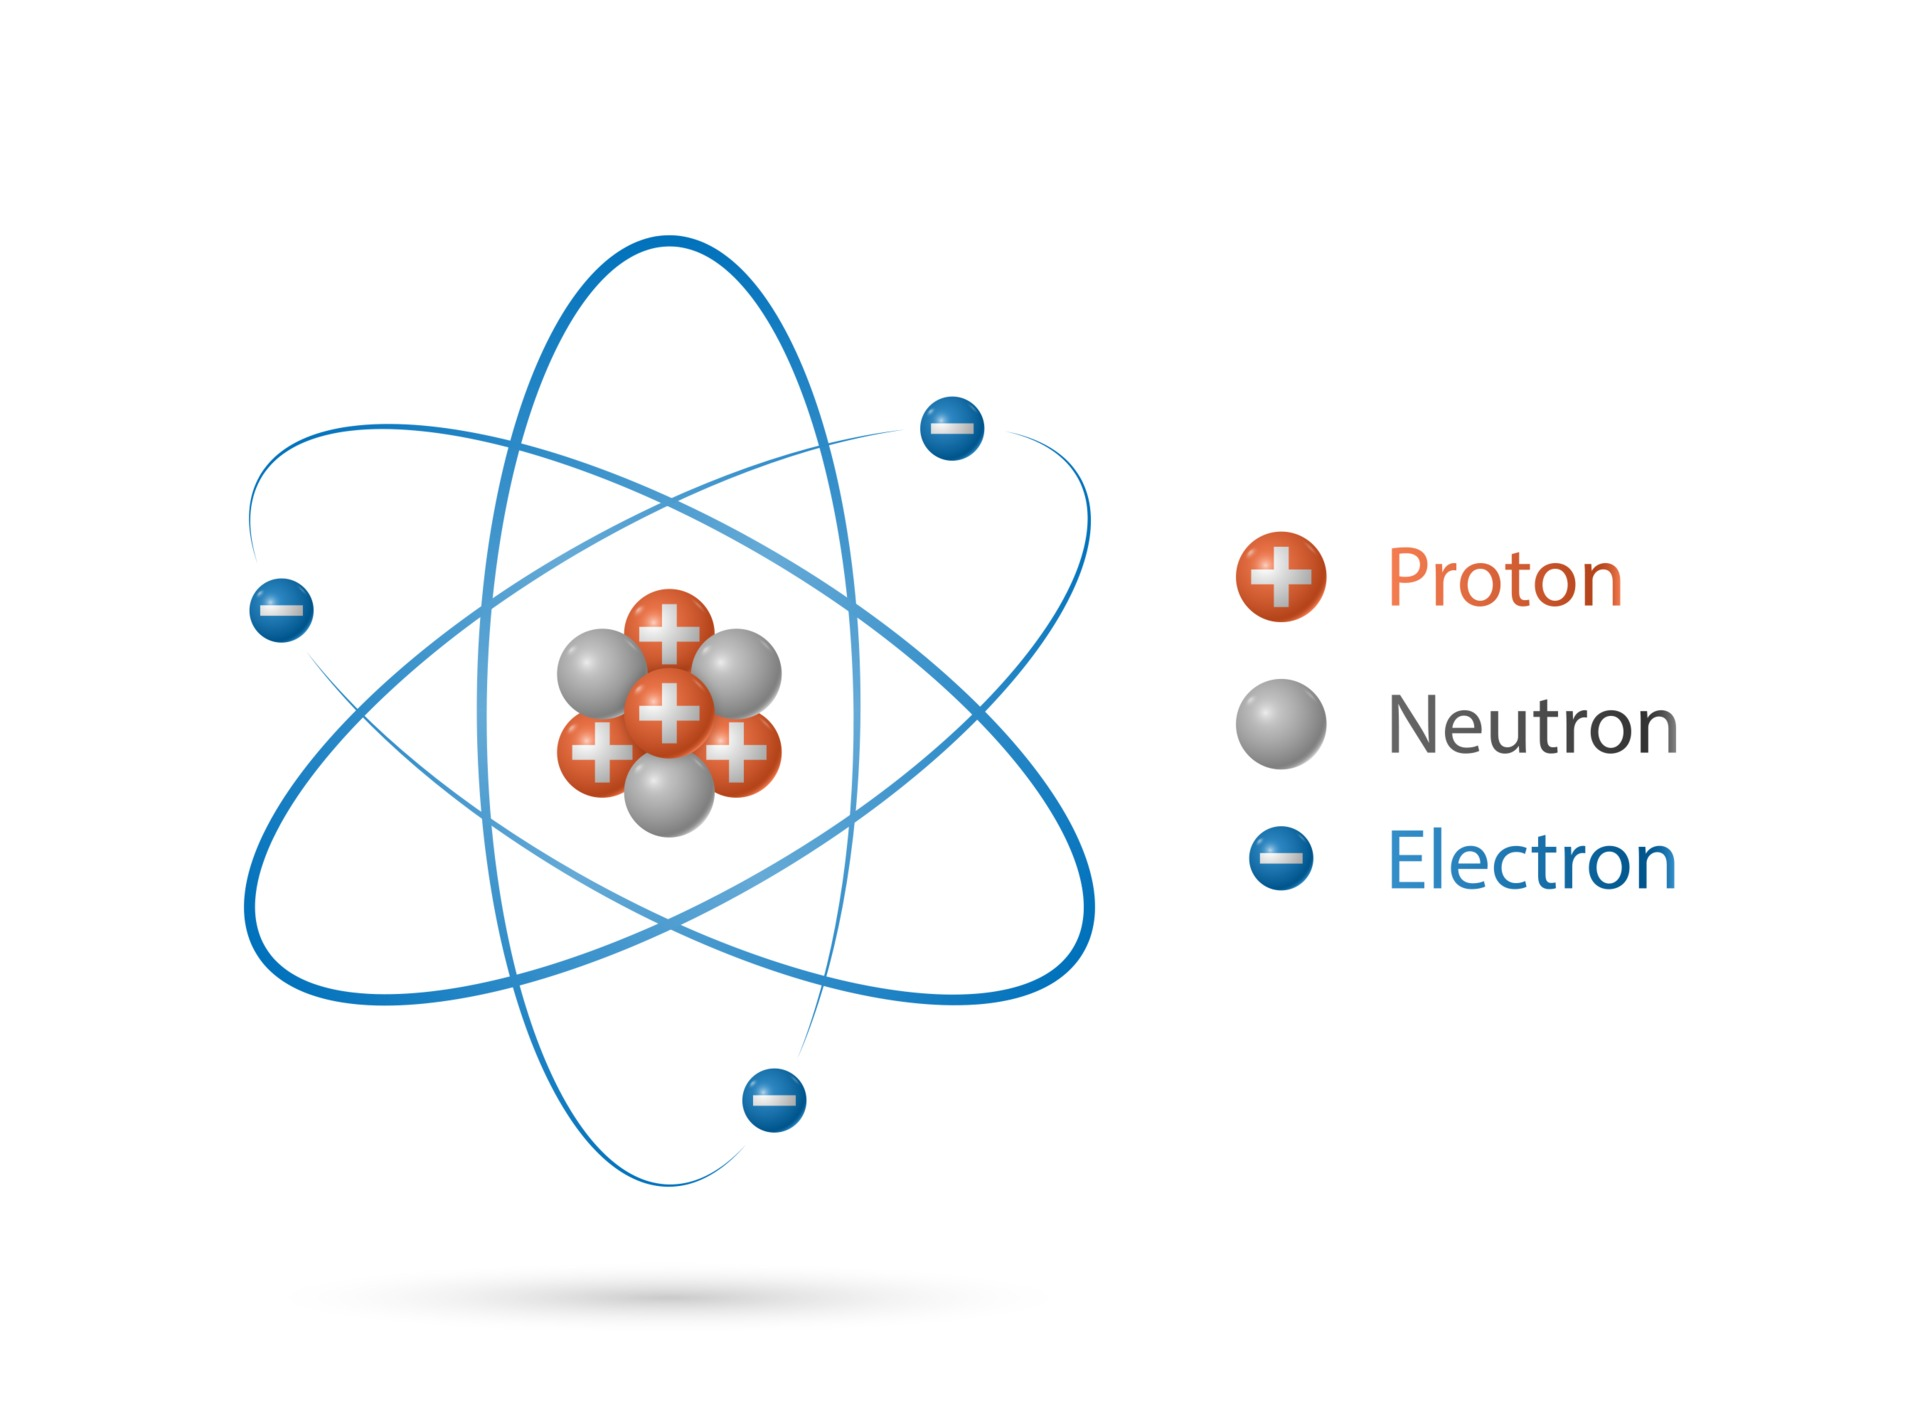
\includegraphics[width=0.4\textwidth]{images/atom_struct.jpg}
    \caption{Estructura básica de un átomo.}
    \label{fig:atom_struct}
\end{figure}

Esta estructura corresponde a un \textbf{modelo atómico}, que es una representación que nos ayuda a entender cómo está compuesto un átomo y cómo se comporta. A lo largo del tiempo han existido distintos modelos atómicos, pero uno de los más conocidos es el \textbf{modelo de Bohr}. Según este modelo, los electrones giran alrededor del núcleo en \textbf{órbitas circulares}, cada una con un nivel de energía específico. Cuando un electrón cambia de órbita, absorbe o emite energía en forma de luz.

La carga elemental \colorbox{highlight}{\( e \)} es la \textbf{cantidad más pequeña de carga eléctrica libre que se conoce en la naturaleza}. Es la carga que poseen los protones y electrones, pero con signo opuesto:

\begin{itemize}
    \item \textbf{Electrón}: \( -e = -1.602 \times 10^{-19} \) C (coulombs)
    \item \textbf{Protón}: \( +e = 1.602 \times 10^{-19} \) C
\end{itemize}

La carga elemental es fundamental porque todas las cargas eléctricas observadas en la naturaleza son \textbf{múltiplos enteros de \( e \)}. Es decir, cualquier carga presente en un objeto es el resultado de un exceso o déficit de electrones. Este principio se conoce como la \textbf{ley de conservación de la carga eléctrica}, y establece que la carga eléctrica \textbf{no se crea ni se destruye}, solo se transfiere de un cuerpo a otro.  

Los objetos tienen carga debido a la presencia de \textbf{electrones y protones}. Un objeto es eléctricamente neutro cuando tiene igual número de ambos. Si un objeto adquiere carga negativa, significa que ha \textbf{ganado electrones}, y si adquiere carga positiva, significa que ha \textbf{perdido electrones}. Cuando un objeto se carga, no se están creando nuevas cargas, sino que \textbf{se están moviendo electrones} de un cuerpo a otro. Por ejemplo: en la \textbf{electrización por frotamiento}, un material transfiere electrones a otro, dejando uno cargado positivamente y el otro negativamente. En la \textbf{inducción}, un objeto cargado puede redistribuir las cargas en otro sin tocarlo, pero sin cambiar la cantidad total de carga en el sistema.

En otras palabras, la carga eléctrica siempre se conserva porque \textbf{los electrones y protones no se destruyen en procesos normales}, solo cambian de ubicación dentro de un sistema.

\colorbox{highlight}{Denominaremos con la letra \( Q \) o \( q \) a la carga eléctrica de un objeto.} La carga se mide en \textbf{coulombs (C)}. Un coulomb es una cantidad de carga muy grande, por lo que en la práctica se utilizan submúltiplos como el \textbf{millicoulomb (mC)} o el \textbf{microcoulomb (\( \mu \text{C} \))}.

\subsection{Fuerza y campo eléctrico}

\subsubsection{Ley de Coulomb}

La electrostática estudia las cargas eléctricas en \hl{\textbf{reposo}}. La ley de Coulomb establece que \textbf{la fuerza entre dos cargas puntuales} es:

\begin{equation}
    F = k_e \frac{\abs{q_1} \cdot \abs{q_2}}{r^2}
    \label{eq:ley_coulomb}
\end{equation}

donde:

\begin{itemize}
    \item \( k_e \) es la constante de Coulomb: \( 8.9876 \times 10^9 \, \frac{\si{\newton\meter\squared}}{\si{\coulomb\squared}} \).
    \begin{itemize}
        \item \( k_e \) se obtiene de  \( \frac{1}{4\pi\epsilon_0} \) y,
        \item \( \epsilon_0 \) es la permitividad del vacío: \( 8.85 \times 10^{-12} \,\frac{\si{\coulomb\squared}}{\si{\newton\meter\squared}} \)
    \end{itemize}
    \item \( q_1 \) y \( q_2 \) son las cargas.
    \item \( r \) es la distancia entre las cargas.
\end{itemize}

Es muy importante notar que la \textbf{Ley de Coulomb} \eqref{eq:ley_coulomb} se aplica estrictamente a \hl{cargas puntuales}, es decir, cargas que se consideran concentradas en un solo punto sin dimensiones espaciales. En la ecuación anterior \eqref{eq:ley_coulomb}, se obtiene la magnitud de la fuerza eléctrica. La expresión vectorial de la fuerza eléctrica es:

\begin{equation}
    \vec{F}_e = k_e \frac{|q_1 q_2|}{r^2} \hat{r}
    \label{eq:ley_coulomb_vectorial}
\end{equation}

donde:
\begin{itemize}
    \item \( \vec{F}_e \) es el vector fuerza eléctrica entre dos cargas puntuales \( q_1 \) y \( q_2 \)
    \item \( \hat{r} \) es el vector unitario en la dirección que une ambas cargas.
\end{itemize}

Esto es importante tenerlo en cuenta ya que si se quiere saber la fuerza total sobre una carga \( q \) debido a varias cargas, se debe sumar vectorialmente las fuerzas individuales. La fuerza total sobre una carga \( q \) debido a un conjunto de cargas \( Q_i \) es:

\begin{equation}
    \vec{F} = \sum_i k \frac{|q \cdot Q_i|}{r_i^2} \hat{\mathbf{r_i}}
    \label{eq:ley_coulomb_vectorial_suma}
\end{equation}

\subsubsection{Cargas eléctricas}

La \textbf{carga eléctrica} es una propiedad fundamental de la materia que determina la interacción electromagnética entre partículas. Se trata de una magnitud escalar que puede ser de dos tipos: \textbf{positiva} o \textbf{negativa}. Las partículas con carga del mismo signo se repelen, mientras que las de signo opuesto se atraen.

La unidad de carga eléctrica en el \textbf{Sistema Internacional (SI)} es el \textbf{coulomb (\( \si{coulomb} \))}. La carga elemental está representada por la carga del electrón (\( -e = -1.602 \times 10^{-19} \si{coulomb} \)) y la del protón (\( e = +1.602 \times 10^{-19} \si{coulomb} \)).

\begin{center}
    \setlength{\arrayrulewidth}{1pt}  % Grosor de líneas
    \renewcommand{\arraystretch}{1.3} % Espaciado vertical
    \arrayrulecolor{gray} % Color de líneas

    \begin{tabular}{ c c c }
        \hline
        \rowcolor{asparagus!30}
        \textbf{Partícula}  & \textbf{Carga (\si{C})}           & \textbf{Masa (\si{kg})}   \\ \hline
        Electrón (e)        & \(-e = -1.602 \times 10^{-19}\)   & \(9.109 \times 10^{-31}\) \\
        Protón (p)          & \(+e = +1.602 \times 10^{-19}\)   & \(1.672 \times 10^{-27}\) \\
        Neutrón (n)         & \(0\)                             & \(1.675 \times 10^{-27}\) \\ \hline
    \end{tabular}
\end{center}

\subsubsection{Campo eléctrico}

Para entender la definición del campo eléctrico desde el principio, debemos pensar en cómo se conceptualiza la interacción entre cargas eléctricas y en la necesidad de definir una propiedad del espacio que describa esta interacción.

Sabemos que las cargas eléctricas ejercen fuerzas unas sobre otras. Experimentalmente, se observa que cargas del mismo signo se repelen y cargas de signo opuesto se atraen. Esta interacción fue formulada matemáticamente por la Ley de Coulomb \eqref{eq:ley_coulomb_vectorial}, sin embargo, esta ley solo nos dice cómo una carga afecta a otra en particular, \hl{pero no describe una propiedad del espacio en sí}. Aquí es donde se introduce el concepto de \textbf{campo eléctrico}.

\begin{figure}[ht]
    \centering
    
\includegraphics[width=0.4\textwidth]{images/field_concept.png}
    \caption{Concepto de campo eléctrico.}
    \label{fig:concepto_campo_electrico}
\end{figure}

En lugar de pensar que una carga actúa instantáneamente sobre otra, se puede imaginar que una carga genera algo en el espacio a su alrededor que luego interactúa con otras cargas. Este ``algo'' es el \textbf{campo eléctrico}. La idea es la siguiente:

\begin{enumerate}
    \item Una carga fuente \( Q \) modifica el espacio circundante.
    \item Cualquier otra carga \( q \) que se coloque en ese espacio experimentará una fuerza debido a esta modificación.
    \item Para cuantificar esa modificación, definimos el campo eléctrico como la \textbf{fuerza por unidad de carga de prueba}.
\end{enumerate}

\paragraph{Idea conceptual del campo eléctrico}

Si te preguntas qué es el campo eléctrico, puedes responder según la descripción previa: ``el campo eléctrico es una propiedad del espacio que rodea a una carga eléctrica capaz de interactuar con otras cargas''. Sin embargo la idea es entender qué significa que una carga eléctrica modifique las propiedades del espacio que la rodea. Veamos un ejemplo de esto para entenderlo mejor.

Supongamos que tengo una carga positiva (un protón) y quiero que se quede totalmente quieto. Entonces ¿Cómo podemos lograr esto? 
Bueno, pues es bastante sencillo. Buscamos alguna carga \( Q \) que a una distancia \( r \) haga que la carga \( q \) del protón anule las fuerzas que interactúan con la carga.

Supongamos que la única fuerza que está interactuando con el protón es la fuerza peso. Entonces tendriamos que encontrar cualquier combinación de \( Q \) y \( r \) que cumpla:

\[
    F_g = F_e = k_e \frac{Q \cdot q}{r^2}
\]

Como nuestras incógnitas son \( Q \) y \( r \) vamos a tener infinitas posibilidades que solucionan muestro problema. Pero antes de dar por terminado el problema te pregunto ¿Qué tienen en común todas las soluciones?

Todas las soluciones están ocacionando el mismo efecto en el protón, una fuerza vertical y hacia arriba (en sentido opuesto al peso). Podriamos expresar esto diciendo: ``todas las soluciones generan una perturbación identica en el punto del espacio donde se encuentra el protón''. O, en otras palabras, todas las soluciones generan un campo eléctrico de las mismas características en donde está el protón.

Es más, cualquier partícula que coloquemos en el lugar del protón, con cualquier carga, por ejemplo una partícula con tres veces la carga del protón pero negativa, sentirá una fuerza proporcional a la que sentía el protón. En el caso de este ejemlo sería una fuerza igual a tres veces el peso del protón en el mimo sentido al peso (por ser negativa).

\paragraph{Formulando el Campo Eléctrico}

El campo eléctrico \( \vec{E} \) se define como la fuerza por unidad de carga de prueba \textbf{positiva} en un punto en el espacio. Esto puede expresarse como:

\begin{equation}
    \vec{E} = \frac{F}{q^{+}} = k_e \frac{Q}{r^2}
\end{equation}

donde:
\begin{itemize}
    \item \( Q \) es la carga que genera el campo (puntual).
    \item \( r \) es la distancia entre la carga de prueba y \( Q \).
\end{itemize}

En caso de que exista más de una carga que genera el campo, se aplica \textbf{el principio de superposición} que consiste en sumar todos todos los campos vectorialmente.

\[
\vec{E} = \sum{\vec{E}_i} = k \cdot \sum{\frac{Q_i}{r^2_i}} \hat{r}_i
\]

En muchos casos, tenemos una distribución continua de carga en vez de una colección de cargas discretas. En esta situación, la carga puede estar distribuida a lo largo de una recta, sobre alguna superficie, por todo un volumen. Siguiendo el concepto de superposición de cargas tendríamos:

\[
\vec{E} = k \lim_{\Delta q_i \to 0} \sum_i{\frac{\Delta q_i}{r_i^2}\hat{r}_i} = k \int \frac{dq}{r^2} \hat{r}
\]

En los casos que debemos calcular el campo de una distribución continua tendremos la \textit{densidad de carga}. Pero ¿Qué es la densidad de carga?

La \textbf{densidad de carga} es una \textit{medida de cuánta carga eléctrica hay distribuida} sobre una determinada región del espacio. Se utiliza cuando las cargas no están concentradas en puntos, sino \textbf{distribuidas} sobre líneas, superficies o volúmenes.

Dependiendo del tipo de distribución, hay tres formas principales:

\subparagraph{1. Densidad lineal de carga:}

Se usa cuando la carga está distribuida a lo largo de una línea (como un alambre).

\[
\lambda = \frac{Q}{l} ~ ~ \rightarrow ~ ~ dq = \lambda dl
\]

\begin{itemize}
    \item \( \lambda \): densidad lineal (C/m)  
    \item \( Q \): pequeña cantidad de carga  
    \item \( l \): pequeña longitud del alambre  
\end{itemize}

\subparagraph{2. Densidad superficial de carga:}

Se usa para cargas sobre una superficie (como una lámina metálica cargada).

\[
\sigma = \frac{Q}{A} ~ ~ \rightarrow ~ ~ dq = \sigma dA
\]

\begin{itemize}
    \item \( \sigma \): densidad superficial (C/m²)  
    \item \( Q \): carga sobre un área pequeña  
    \item \( A \): área considerada  
\end{itemize}

\subparagraph{3. Densidad volumétrica de carga:}

Se usa cuando la carga ocupa un volumen (como una nube de plasma).

\[
\rho = \frac{Q}{V} ~ ~ \rightarrow ~ ~ dq = \rho dV
\]

\begin{itemize}
    \item \( \rho \): densidad volumétrica (C/m³)  
    \item \( Q \): carga dentro de un pequeño volumen  
    \item \( V \): volumen correspondiente  
\end{itemize}


Estas densidades permiten convertir una distribución continua de carga en una integral, y así calcular el campo eléctrico o el potencial.  
Por ejemplo, si conocés \( \lambda(x) \), podés calcular el campo eléctrico de una varilla cargada mediante:

\[
\vec{E} = \frac{1}{4\pi\varepsilon_0} \int \frac{\lambda(x)\, dx}{r^2} \hat{r}
\]

\paragraph{Visualización del campo eléctrico}

Para visualizar el campo eléctrico veamos un ejemplo sencillo. Supongamos que tenemos tres cargas eléctricas de distinto valor ubicadas en tres lugares distintos. Todas estas cargas están fijas en su posición y no pueden moverse (ver figura \ref{fig:campo_electrico_ejemplo_1}). 

\begin{figure}[ht]
    \centering
    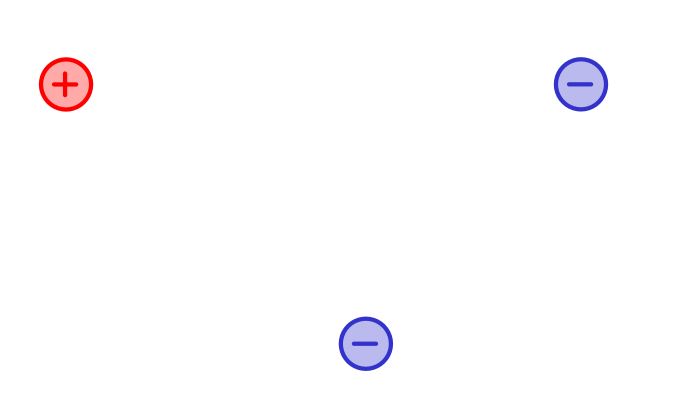
\includegraphics[width=0.5\textwidth]{images/field_ex_1.png}
    \caption{tres cargas fijas en el espacio.}
    \label{fig:campo_electrico_ejemplo_1}
\end{figure}

Estas tres cargas posicionadas en el espacio constituyen lo que llamaremos \textbf{carga fuente}. Estas tres cargas fuente son capaces de generar una fuerza en cualquier partícula con carga que se coloque en este espacio. Podemos decir entonces, que las tres cargas le dan una propiedad eléctrica al espacio que las rodea. A esta propiedad que adquiere el espacio por culpa de las cargas le llamaremos campo eléctrico y existe independientemente de que haya otra cuarta carga presente o no.

Ahora supongamos que queremos jugar con el campo generado, y tomamos una cuarta carga \( q^{+} \), en este caso la carga será positiva, y la llamaremos \textbf{carga de prueba}. Entonces colocamos la carga de prueba en el centro de las tres cargas y la soltamos (ver figura \ref{fig:campo_electrico_ejemplo_2})

Cuando la soltamos, la carga será empujada hacia algún lugar, ya que, experimentará una fuerza debido a la interacción con las otras cargas. Ya sabemos que las cargas del mismo signo se repelen y las de signo opuesto se atraen.

\begin{figure}[ht]
    \centering
    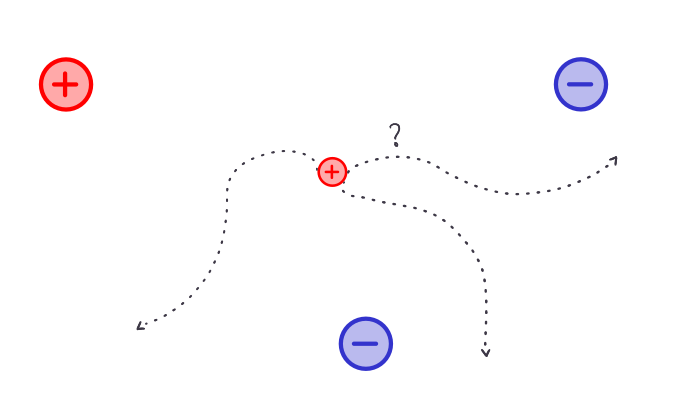
\includegraphics[width=0.5\textwidth]{images/field_ex_2.png}
    \caption{colocamos una cuarta carga en el centro y la soltamos.}
    \label{fig:campo_electrico_ejemplo_2}
\end{figure}

Entonces aquí tenemos tres cargas aplicando tres fuerzas distintas, ¿qué hacemos? Sumar todas las fuerzas. Algunas se van a contrarrestar un poco al estar en direcciones opuestas, pero otras se van reforzar al tirar en el mismo sentido.

La suma de todas estas fuerzas (fuerza resultante) nos indica hacia dónde va ir la carga y la intensidad del empujón que sentirá (magnitud de la fuerza). Si realizamos esto en cada punto del espacio acabaríamos llenando el espacio de vectores de fuerza, esto se vería como un ``mapa de flechas'' que representan la fuerza que siente la carga de prueba en cada punto.

\textbf{Pero espera:} imaginemos que realizamos todos los cálculos con una carga de prueba de \( 1 \si{\coulomb} \). Y esa carga de prueba en realidad solo la usamos para realizar los cálculos del mapa, pero en realidad no existe. Entonces este mapa lo podemos usar para saber qué fuerza sentiría una carga \( q \) cualquiera.
Seguro te preguntarás ¿Cómo es eso? Es bien sencillo, presta atención a lo siguiente. Si recordamos la ecuación de la fuerza debido a la interacción entre cargas tenemos:

\[
\vec{F}_e = k\frac{Q\cdot q^{+}}{r^2}\hat{r} 
\]

Ahora, recordando que \( Q \) era nuestra carga fuente (formada por las tres cargas) y \( q^{+} \) nuestra carga de prueba de \( 1 \si{\coulomb} \) que usamos para hacer todas las cuentas, si quitamos la carga de prueba, como en la ecuación de fuerza es un factor neutro (multiplica por 1), el resultado no cambiaría cuantitativamente, sin embargo cambiarían las unidades. Veamos como queda:

\[
\vec{F}_e ~ [\si{\newton}] \neq k \frac{Q}{r^2} \hat{r} ~ [\si{\newton\per\coulomb}]
\]

Vemos que lo que resulta es una desigualdad, ya que las unidades no coinciden. Si bien numericamente es lo mismo, dimensionamente no. Para arreglar este problema entonces, en vez de quitar directamente la carga, podemos dividir ambos miembros por \( q^{+} \), y no romperíamos las unidades:

\[
\frac{\vec{F}_e}{q^{+}} ~ [\si{\newton\per\coulomb}] = k \frac{Q}{r^2} \hat{r} ~ [\si{\newton\per\coulomb}]
\]

\begin{figure}[ht]
    \centering
    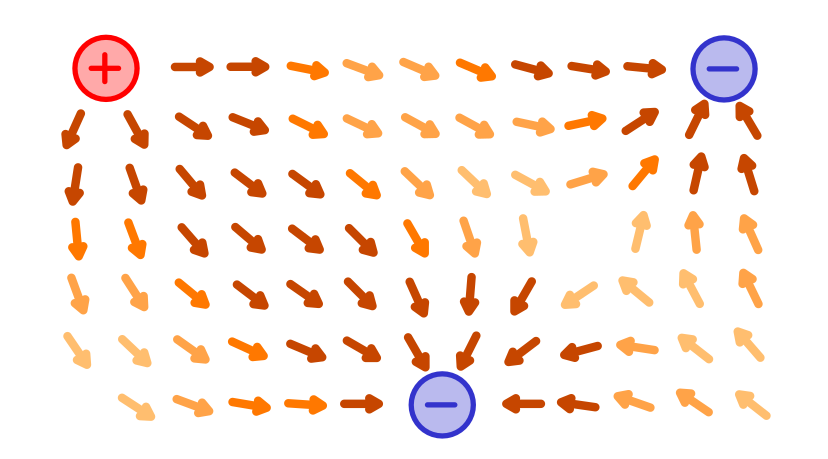
\includegraphics[width=0.5\textwidth]{images/field_example.png}
    \caption{mapa de la fuerza que siente \(q^{+}\) en cada punto.}
    \label{fig:campo_electrico_ejemplo_3}
\end{figure}

¿Qué nos dice este ``mapa de flechas''? Este mapa de flechas nos dice la \hl{fuerza por unidad de carga} que generan las cargas fuente. Es decir, si colocamos una carga unidad (como \(q^{+}\)), entonces la relación es \(1:1\), pero podemos colocar cualquier carga \(q\) y multiplicarla por el campo.

\begin{equation}
    \vec{E} = \frac{\vec{F}}{q^{+}}
    \label{eq:campo_electrico}
\end{equation}

donde:
\begin{itemize}
    \item \( \vec{E} \) es el campo eléctrico en ese punto,
    \item \( \vec{F} \) es la fuerza experimentada por la carga de prueba \( q^{+} \),
    \item \( q^{+} \) es la carga de prueba.
\end{itemize}

Ahora, como vimos, la carga de prueba es una carga hipotética utilizada para medir el campo sin modificarlo. Como la carga de prueba es positiva, entonces vemos que una carga \(Q\) cualquiera, respeta la siguiente distribución: si la carga \(Q\) es \textbf{negativa}, las líneas de campo son entrantes, si la carga \(Q\) es \textbf{positiva}, las líneas de campo son salientes:

\begin{figure}[ht]
    \centering
    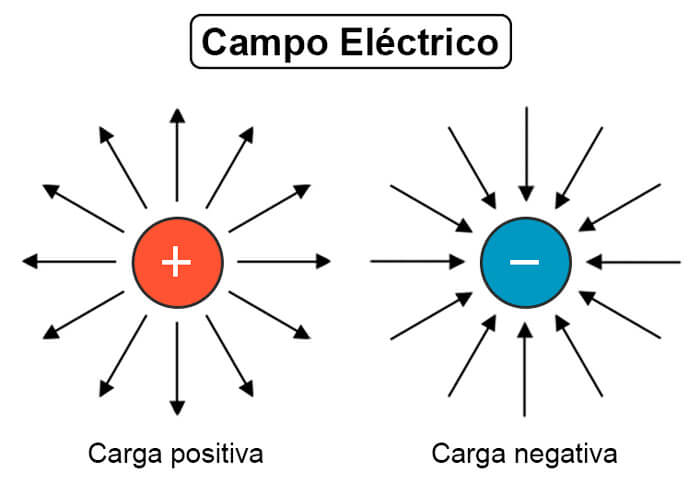
\includegraphics[width=0.5\textwidth]{images/electric_field.jpg}
    \caption{Campo eléctrico de una carga puntual positiva y una negativa.}
    \label{fig:campo_electrico}
\end{figure}

Este resultado nos dice que el campo eléctrico \textbf{se aleja} de cargas positivas y \textbf{se dirige hacia} cargas negativas. Además disminuye con el cuadrado de la distancia y es una propiedad del espacio ya no depende de la carga de prueba \( q \), sino solo de \( Q \).

Es muy importante tener en cuenta las premisas usadas para formular el \textbf{campo eléctrico}:
\begin{itemize}
    \item \textit{La carga fuente modifica el espacio circundante:} El campo eléctrico es una propiedad del espacio y es generado por una carga fuente.
    \item \textit{El campo es independiente de la carga de prueba:} La carga de prueba se usa solo como herramienta de medición.
    \item \textit{El campo es un campo vectorial:} Tiene dirección y magnitud en cada punto del espacio.
    \item \textit{El campo sigue el principio de superposición:} Si hay varias cargas, el campo total en un punto es la suma vectorial de los campos generados por cada una.
    \item \textit{La carga de prueba es positiva:} Para determinar el sentido del campo es importante tener en cuenta que la carga de prueba es positiva, esto permite ver con claridad cuando el campo es entrante o saliente para una carga puntual, o poder predecir correctamente el sentido del campo en una distribución de cargas (ya sea discreta o continua).
\end{itemize}

\subsubsection{Lineas de campo eléctrico}

Las líneas de campo no son más que un medio para visualizar el patrón formado por el campo eléctrico a través del trazo de líneas conocidas como \textbf{líneas de campo eléctrico}. Estas líneas relacionan el campo eléctrico con una región del espacio de la siguiente manera:
\begin{itemize}
    \item El vector \(\vec{E}\) del campo eléctrico es tangente a la línea del campo eléctrico en cada punto y la dirección de la linea de campo es igual a la del campo eléctrico.
    \item El número de líneas de campo que pasan por una superficie perpendicular a dichas líneas es proporcional a la magnitud de campo.
\end{itemize}

\begin{figure}[ht]
    \centering
    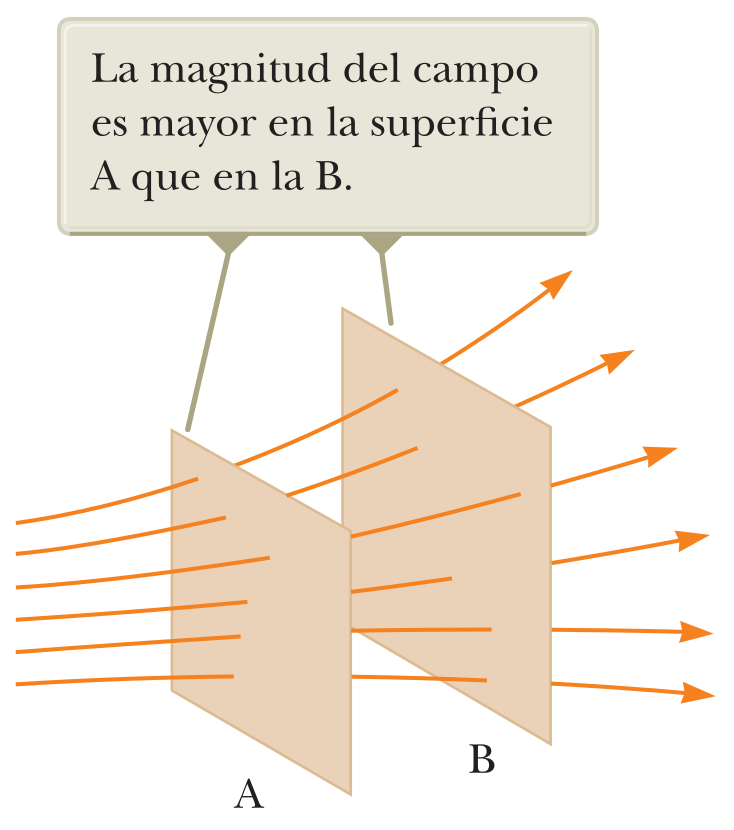
\includegraphics[width=0.5\textwidth]{images/field-lines.png}
    \caption{Líneas de campo eléctrico que atraviesan dos superficies}
    \label{fig:lineas_de_campo}
\end{figure}

Pongamos este concepto en palabras simples ¿Recuerdas el ejemplo de las tres cargas y el ``mapa de flechas''? Bueno, las líneas de campo nos ayudan a visualizar el ``mapa de flechas'' de una forma más cómoda.

\begin{figure}[ht]
    \centering
    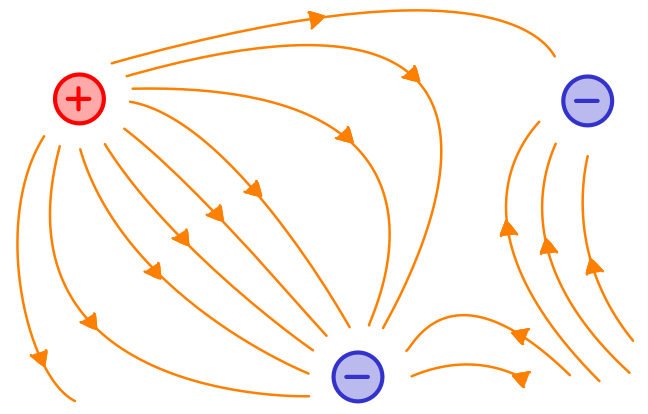
\includegraphics[width=0.5\textwidth]{images/field_lines_ex.png}
    \caption{Ejemplo del ``mapa de flechas'' visualizado con líneas de campo}
    \label{fig:ej_lineas_de_campo}
\end{figure}

En este caso se puede ver que las líneas de campo están más juntas cuando nos acercamos a las cargas, y se van separando cuando nos alejamos. La proximidad entre líneas de campo nos indica que el campo es intenso. Si las líneas están distantes entre sí indica que el campo es menos intenso. Esto se puede verificar con la ecuación del campo eléctrico, ya que el campo disminuye con el cuadrado de la distancia. Esto significa que según más nos alejamos de las cargas fuente, el campo disminuye.

\subsection{Flujo eléctrico}

La ley de Gauss es uno de los principios fundamentales del electromagnetismo y proporciona una forma muy poderosa de calcular el campo eléctrico en situaciones con simetría.

La ley de Gauss dice:
\begin{equation}
    \Phi_E = \oint_{\text{superficie cerrada}} \vec{E} \cdot d\vec{A} = \frac{q_{\text{int}}}{\varepsilon_0}
\end{equation}

donde:
\begin{itemize}
    \item \( \Phi_E \) es el flujo de campo eléctrico a través de una superficie cerrada.
    \item \(E\) es el campo eléctrico en cada punto de esa superficie.
    \item \(dA\) es un vector diferencial de área que apunta hacia afuera de la superficie.
    \item \(q_{int}\) es la carga total encerrada dentro de la superficie.
    \item \(\epsilon_0\) es la permitividad del vacío, una constante del medio.
\end{itemize}

\paragraph{¿Qué nos dice esta ley, en términos simples?}

El flujo eléctrico representa la cantidad de ``líneas de campo eléctrico'' que atraviesan una superficie.

Si hay carga dentro de una superficie cerrada, el campo eléctrico "sale" (o "entra") por esa superficie, generando un flujo distinto de cero.

Si no hay carga neta dentro, el flujo eléctrico total es cero, aunque el campo pueda no ser nulo en todos los puntos.

No importa la forma de la superficie: solo importa cuánta carga encierra, no cómo se distribuye el campo en detalle.

\subparagraph{¿Por qué es útil la ley de Gauss?}

La ley de Gauss es útil porque, en situaciones con alta simetría (esférica, cilíndrica, planar), permite calcular el campo eléctrico sin integrar la ley de Coulomb.

Por ejemplo:
\begin{itemize}
    \item Una esfera cargada uniformemente
    \item Un hilo largo con carga lineal uniforme
    \item Un plano infinito cargado
\end{itemize}

En estos casos, elegir una superficie cerrada adecuada (llamada superficie gaussiana) permite calcular  de forma directa.

\subparagraph{Ejemplo clásico: esfera cargada}

Supón una carga  distribuida uniformemente en una esfera. Si elegimos una superficie esférica de radio  mayor al de la esfera, por simetría:
\[
\vec{E} = \text{constante} \quad \text{y} \quad \vec{E} \parallel d\vec{A}
\]
Entonces la integral se simplifica:
\[
\oint \vec{E} \cdot d\vec{A} = E \oint dA = E(4\pi r^2)
\]
Y por la ley de Gauss:
\[
E(4\pi r^2) = \frac{Q}{\varepsilon_0} \quad \Rightarrow \quad E = \frac{1}{4\pi\varepsilon_0} \frac{Q}{r^2}
\]
¡Y así recuperamos la fórmula del campo eléctrico de una carga puntual!


\input{chapters/2_direct_current.tex}
\input{chapters/3_electromagnetism.tex}
\input{chapters/4_waves_and_vibrations.tex}
\input{chapters/5_optics.tex}
\input{chapters/6_intro_of_fluids.tex}
\input{chapters/7_dynamic_of_fluids.tex}
\input{chapters/8_heat_and_temperature.tex}

\end{document}
